%\documentclass[aps,pre,superscriptaddress,floatfix,11pt]{revtex4-1}

%
\documentclass[11pt]{amsart}
%\usepackage{geometry}                % See geometry.pdf to learn the layout options. There are lots.
%\geometry{letterpaper}                   % ... or a4paper or a5paper or ... nd{document}  \documentclass[11pt,A4,showpacs]{amsart}
\usepackage{amsmath,amsfonts,amssymb}
\usepackage{graphicx}

%\usepackage{wrapfig}
\usepackage{algorithm}
\usepackage{algorithmic}
\usepackage{epstopdf}
%\usepackage{ulem}
\usepackage{float,placeins}
\usepackage[hyperfigures,breaklinks,colorlinks,citecolor=blue,linkcolor=black]{hyperref}
%\usepackage[justification=raggedright]{caption}
\usepackage{subfigure}
%\usepackage[caption=false]{subfig}
\usepackage{mathbbol}

\usepackage{amsmath,amsfonts,amssymb}
\usepackage{amsthm}
\usepackage{graphicx}
\usepackage{hyperref}
\usepackage{pstricks}
\usepackage{amsmath}
\theoremstyle{definition} \newtheorem{defi}{Definition}


%\usepackage{listings}	% for inserting program code
\setlength{\parskip}{1em}

\def\s{\sigma}
\def\ul{\underline}
\def\p{\partial}
\DeclareMathOperator{\sign}{sign}

\newcommand{\la}[1]{\lambda_{#1}}
\newcommand{\lasub}[3]{\lambda_{#1 \rightarrow (#1 #2)} [\sigma_{#1}(#3),\sigma_{#2}(#3),#3]}
\newcommand{\lasubX}[3]{\lambda_{#1 \rightarrow (#1 #2)} [X_{#1},X_{#2},#3]}
\newcommand{\lasubsim}[3]{\lambda_{#1 \rightarrow (#1 #2)} (#3)}
\newcommand{\musubsim}[3]{    \mu_{#1 \rightarrow (#1 #2)} (#3)}
\newcommand{\musub}[3]{    \mu_{#1 \rightarrow (#1 #2)} (X_{#1}(#3)|X_{#2}(#3))}
\newcommand{\musubX}[2]{    \mu_{#1 \rightarrow (#1 #2)}(X_{#1}|X_{#2})}



\begin{document}
\title{Low Auto-correlation Binary Sequences explored using Survey Propagation}

\date{\today}

\begin{abstract}
  \noindent
TODO

\end{abstract}
\maketitle

\section{Introduction}

The Low Auto-correlation Binary Sequence (LABS) problem consists in finding a binary sequence $ S =\{S_1, S_2,..., S_N\} $ where $ S_i \in \{1,-1\}  $ for $1\leq i \leq N$ that minimizes the function
\begin{equation}
E(S)=\sum_{k=1}^{N-1}C_k(S)^2 \label{eq:energy}
\end{equation}
\noindent where $C_k(S)$ are the aperiodic auto-correlation coefficients:
\begin{equation}
C_k(S)=\sum_{i=1}^{N-k} S_i S_{i+k}, \mbox{ for } 1 \leq k \leq N-1. \label{eq:autocorr}
\end{equation}
\noindent Finding such optimal sequences is a notoriously hard problem, for increasing values of $N$\cite{bovskovic14}.

To build these low auto-correlation binary sequences is of fundamental interest in many practical applications. In radars, for example, LABS are required for modulation in the process of pulse compression to enhance range resolution and long range detection capabilities \cite{SR14}. Also for the measurement of space-time curvatures between high precision radars \cite{Mertens16}.
In Mathematics it is known as the Littlewood problem, that consists in finding the coefficients of a polynomial around the unit circle in the complex plane.
In Statistical Physics, these are the ground states of the Bernasconi's model \cite{Bernasconi87}, that implies the energy minimization of an Ising spin system with long range interacting variables with four-fold antiferromagnetic interactions.
Morover, it also appears in digital signaling processing \cite{Kratica12}, and in Artificial Inteligence \cite{Amaya13}.

The problem has been largely studied using exact and heuristic methods. Exhaustive search is currently the only available way to obtain exact LABS solutions. 
Golay published in \cite{Golay} optimal solutions for values up to $N = 32$. Since then, due the computational complexity of the problem, all the new optimal solutions have been obtained using Branch and Bound \cite{Mertens16} methods with different parallel implementations, resulting in algorithms with cost of order $O(k^N )$ with $k < 2$.

For example, Mertens found the solution of the LABS problem up to $N \leq 48$ with a computational cost of $O(1.85^N)$ in 1996 \cite{Mertens96}.
Later in 2004 with an improved implementation Mertens and Bauke computed the solution up to $N \leq 60$ \cite{Mertens16}. 
Wiggenbrock expanded this approach to $N \leq 64$ using a better bound and reported a cost of order $O(1.79^N)$ \cite{Mertens16}.
More recently in 2016, Packebusch and Mertens obtained exact solutions for two more values $N = 65$ and $N = 66$, employing the combined bounds of Prestwich and Wiggenbrock $O(1.729^N)$ \cite{Mertens16}.
Despite these sophisticated implementations and improvements it is clear that this approach is not viable in the search of optimal sequences with larger lengths, for example, $N > 100$.

A readable summary of the application of different heuristic and stochastic algorithms to LABS appears in  \cite{Amaya13} and \cite{bovskovic14}.
More specifically, in \cite{Militzer} the authors used  Evolutionary Search (ES) taking a special care on processes to generate the offsprings without a recombination strategy and with a mutation operator flipping more than one bit at once, the authors found solutions, for odd system sizes, as large as $N = 201$.
In \cite{Gallardo} the authors presents empirical evidence showing that evolutionary pure algorithms are not capable of facing the complexity of the problem, but also that evolutionary methods assisted by local-search operators (memetic algorithms) provide optimal or near-optimal results.
In \cite{Halim} the authors improved the Tabu Search Method previously developed in \cite{Dotu} getting better results than memetic algorithms and they explore the solution space for systems size between $[61-77]$ and report the best values that they obtain with TSv7 algorithm which has an expected run time of $\mathcal{O}( 1.03\mathrm{e}{-5} \cdot 1.34^N)$,  according to these authors the improvement came from a deep study of the searched trajectories and a better diversification process.
The state of the art of heuristic algorithms according to \cite{Mertens16} seems to be the work \cite{bovskovic14} where the authors combined a random self-avoiding walk and Hasse graph.
However, like with exact algorithms these complex and advanced heuristics fail in systems of relative high dimensions \cite{Mertens16} leaving room for further improvements.

Here we first introduce Warning Propagation and compare it to Greedy Monte Carlo, to show that indeed, it is a better candidate to look for low energy configurations of the LABS problem. 
Then we try WP on the disordered versions of LABS in order to shed light on the relevance of the structure for the underlying graph of interactions on the space of available configurations of the problem.

\section{Physically inspired algorithms}

The minimization of the energy $E(S)$ (cost function) can be obtained by specific methods tailored for this very problem, as
those that are the state of the art for LABS, or conversely by general standard techniques. While the former are currently more efficient
the later are easier to interpret and  may open the way to important new ideas in the treatment of the problem.
The simplest of these algorithms is the greedy minimization of the cost function. A simple greedy approach corresponds in the statistical mechanics community
to the Monte Carlo method at $T=0$, where variables are iteratively altered only when the proposed changes reduce the energy.
Typically greedy algorithms are simple to program and guaranteed to converge, but are prone to get stuck on non-optimal solutions.

On the other hand, since the beginning of the century,  Message Passing algorithms have found their way in the realm of the statistical physics community.
The turning point was the realization that message passing algorithms can be viewed as fixed point equations derived from variational approximations to the free energy of Ising-like models \cite{Yedidia02}.
This inspired researchers to look for novel applications of these algorithms in the field of Combinatorial Optimization \cite{Mulet02, Braunstein03, Weigt06} and to explore new extensions \cite{SP,CVM,GBP}.

\section{Survey Propagation}

	\begin{equation}
	u_{a \to i}=sgn(- h_j h_k h_l)min(|-1|,|h_j|,|h_k|,|h_l|)
	\end{equation}
	
	\begin{equation}
	P(h_i) = \int_{u}\prod_{a \in V(i)} Q(u_{a\to i})
	\delta(h_i -\sum_{i=1}^m u_i) d(u_i)
	\end{equation}

	\begin{multline}
	Q(u_{a \to i}) = \int_{h_j}\int_{h_k}\int_{h_l}P(h_j)P(h_k)P(h_l)
	\\
	\delta(u-sgn(- h_j h_k h_l)min(1,|h_j|,|h_k|,|h_l|))dh_j dh_k dh_l
	\end{multline} 

	Debido a que estamos lidiando con valores discretos de $u$ y $h$ es util asumir que:

	\begin{equation}
	Q(u_{a \to i}) = \eta_0 \delta(u_{a \to i}) + 
	\eta_1 \delta(u_{a \to i}-1) + 
	\eta_{-1} \delta(u_{a 	\to i} + 1)
	\end{equation}
	
	y por ende
	
	\begin{multline}
	P(h_i) = \rho_0 \delta(h_i) + \rho_1 \delta(h_i - 1) + 
	\rho_{-1} \delta(h_i + 1) + ...
	\\
	\rho_n \delta(h_i - n) + \rho_{-n} \delta(h_i + n)
	\end{multline} 
	
	en este punto resulta necesario encontrar una relacion entre $\eta$ y $\rho$. 
	\\
	Empecemos por $\eta_0$,
	$\eta_0$ en principio significa la probabilidad de que $u_{a \to i}$ 
	tome valor $0$, para que esto ocurra es necesario que el producto del 
	$sgn$ sea $0$ o que el $min$ de los valores absolutos sea $0$. Estas 
	dos condiciones necesitan que una, dos o las tres $h$ involucradas tomen 
	valor cero y esto puede suceder de distintas combinaciones.

	\begin{multline}
	\eta_0^{a \to i} = \rho_0^j \rho_0^k \rho_0^l + 
	\rho_0^j \rho_0^k [\sum_{\alpha \in [-n, n] / 0} \rho_{\alpha}^l]+
	\\
	\rho_0^j [\sum_{\alpha \in [-n, n] / 0} \rho_{\alpha}^k] \rho_0^l+
	[\sum_{\alpha \in [-n, n] / 0} \rho_{\alpha}^j] \rho_0^k \rho_0^l+
	\\
	\rho_0^j[\sum_{\alpha \in [-n, n] / 0} \rho_{\alpha}^k][\sum_{\beta \in [-n, n] / 0} \rho_{\beta}^l]+
	\\
	[\sum_{\alpha \in [-n, n] / 0} \rho_{\alpha}^j] \rho_0^k [\sum_{\beta \in [-n, n] / 0} \rho_{\beta}^l]+
	\\
	[\sum_{\alpha \in [-n, n] / 0} \rho_{\alpha}^j][\sum_{\beta \in [-n, n] / 0} \rho_{\beta}^k]	\rho_0^l
	\end{multline} 

	apoyandonos en que
	
	\begin{equation}
	\sum_{\alpha \in [-n, n] / 0} \rho_{\alpha}^j = 1-\rho_0^j
	\end{equation}
	
	razonando de forma similar para $k$, $l$  y aplicando cierto trabajo algebraico es 
	posible simplificar la expresion anterior hasta obtener:

	\begin{multline}
	\eta_0^{a \to i} = 
	\rho_0^j \rho_0^k \rho_0^l - (\rho_0^j \rho_0^k + \rho_0^k \rho_0^l + \rho_0^j 	\rho_0^l) +
	\\
	\rho_0^j + \rho_0^k + \rho_0^l
	\end{multline} 

	para obtener $\eta_1$ es necesario notar que $sgn(-h_j h_k h_l)=1$, si y 
	solo si $h_j h_k h_l < 0$. Es decir los tres valores de $h$ deben ser negativos o 
	solo uno de estos puede serlo. Por ende:

	\begin{multline}
	\eta_1^{a \to i} = 
	\sum_{\alpha \in [-n, -1]} \rho_{\alpha}^j \sum_{\beta \in [-n, -1]} \rho_{\beta}^k \sum_{\gamma 	\in [-n, -1]} \rho_{\gamma}^k +
	\\
	\sum_{\alpha \in [-n, -1]} \rho_{\alpha}^j \sum_{\beta \in [1, n]} \rho_{\beta}^k \sum_{\gamma \in [1, n]} \rho_{\gamma}^k +
	\\
	\sum_{\alpha \in [1, n]} \rho_{\alpha}^j \sum_{\beta \in [-n, -1]} \rho_{\beta}^k \sum_{\gamma \in 	[1, n]} \rho_{\gamma}^k +
	\\
	\sum_{\alpha \in [1, n]} \rho_{\alpha}^j \sum_{\beta \in [1, n]} \rho_{\beta}^k \sum_{\gamma \in [-	n, -1]} \rho_{\gamma}^k
	\end{multline} 

	la expresion anterior luce complicada, pero sugiere que es posible expresarla 
	como un funcion comulativa de los valores de $\rho$. 
	Sea $C_{-1}^j = \sum_{\alpha \in [-n, -1]} \rho_{\alpha}^j$, sin tener en cuenta 
	los valores individuales de $\rho$.

	\begin{multline}
	\eta_1^{a \to i} = 
	C_{-1}^j C_{-1}^k C_{-1}^l +
	C_{-1}^j C_{1}^k C_{1}^l   +
	\\
	C_{1}^j C_{-1}^k C_{1}^l +
	C_{1}^j C_{1}^k C_{-1}^l
	\end{multline} 

	y por ende: 
	
	\begin{multline}
	\eta_{-1}^{a \to i} = 
	C_{1}^j C_{1}^k C_{1}^l +
	C_{1}^j C_{-1}^k C_{-1}^l   +
	\\
	C_{-1}^j C_{1}^k C_{-1}^l +
	C_{-1}^j C_{-1}^k C_{1}^l
	\end{multline}

	Aplicando el mismo razonamiento anterior podemos derivar las ecuaciones para el 
	modelo de 2-Spin antiferromagnetico.
	\begin{equation}
	\eta_0^{a \to i} = \rho_0^j
	\end{equation}

	\begin{equation}
	\eta_1^{a \to i} = \sum_{\alpha \in [-n, -1]}\rho_\alpha^j
	\end{equation}
	
	\begin{equation}
	\eta_{-1}^{a \to i} = \sum_{\alpha \in [1, n]}\rho_\alpha^j
	\end{equation}

	Queda pendiente el problema de la obtencion de los valores de 
	$C_{-1}$, dado que el computo de este valor depende de un n\'umero 
	largo de t\'erminos $\sum_{\alpha \in [-n, -1]} \rho_{\alpha}^j$ que 
	crece con la dimensi\'on del problema es necesario la obtencion de un 
	m\'etodo para la computacion de este. Estudiaremos dos m\'etodos a continuaci\'on.


\section{Results}

\begin{figure}[h]
\centering
\includegraphics[scale=1]{../prob.eps}
\caption{Probability of found the ground state given partial information. The Y axis is the probability, and X axis is the inverse of the information of the ground state. The Graphic show that, a transition occur around the middle of partial information.} 
\label{fig:Labs_Histogram}
\end{figure}

\begin{figure}[h]
\centering
\includegraphics[scale=1]{../decimate_09.eps}
\caption{Amount of decimate variable with bias values greater than 0.9 . The Y axis a normalization for the lowers curves of system sizes where the bias has a value greater than .9. The graphic show that the amount of spin with no initial set of value, increasing in the same region where the probability of founding the GS  decreasing is 1, and when the amount of this spins decreasing the probability decrease at the same rate.} 
\label{fig:Labs_Histogram}
\end{figure}


\begin{figure}[h]
\centering
\includegraphics[scale=1]{../decimate_07.eps}
\caption{Equal to the second graph, but with the .7 threshold.} 
\label{fig:Labs_Histogram}
\end{figure}

\begin{figure}[h]
\centering
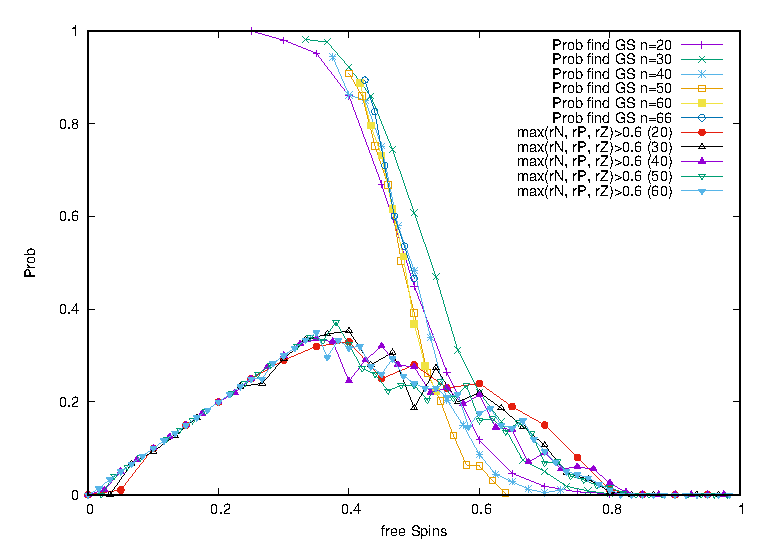
\includegraphics[scale=1]{../decimate_06.eps}
\caption{Equal to the second graph, but with the .6 threshold.} 
\label{fig:Labs_Histogram}
\end{figure}

\begin{figure}[h]
\centering
\includegraphics[scale=1]{../decimate_05.eps}
\caption{Equal to the second graph, but with the .5 threshold.} 
\label{fig:Labs_Histogram}
\end{figure}

\begin{figure}[h]
\centering
\includegraphics[scale=1]{../decimate_01.eps}
\caption{Equal to the second graph, but when the difference between Rho Positive and Rho Negative is bigger than .1} 
\label{fig:Labs_Histogram}
\end{figure}

\bibliographystyle{plain}
\bibliography{bibliolabsv4}

\end{document}
